% !TeX spellcheck = en_US
% !TeX encoding = UTF-8
% !TeX root = ../document.tex

\chapter{Discovery Potential}
\label{chap:sensitivity_studies}

\section{Results}
\label{sec:results}

The following sections will present the results of the analysis of the discovery potential. For each signal model, we will show the most significant classes, distribution of \ptilde values and the newly introduced \phat results which quantify the test power towards a certain model. 
We will start by presenting a validation which has been obtained by executing the entire analysis on a \ac{SM}-only sample.


We will claim to be sensitive to a model if any \phat test power is above \SI{70}{\percent}.

\subsection{Validation Using the \ac{SM}}
\subsubsection{Most Significant Classes}
%\begin{table}
%    \centering
%    \begin{longtable}{l S[table-figures-integer=1,table-figures-decimal=2,table-comparator=true,table-figures-exponent=1] S[table-figures-integer=1,table-figures-decimal=1,table-comparator=true,table-figures-exponent=0]}
\toprule
{Event Class} & {Median \ptilde} & {$Z$} \\
\midrule
\endhead
\num{1} \Pe + \num{1} \Pmu + \MET + X & 2.00e-04 & 3.5 \\
\num{1} \Pe + \num{1} \Pmu + X & 5.00e-04 & 3.3 \\
\num{1} \Pe + X & 1.82e-02 & 2.1 \\
\num{1} \Pe + \num{1} \Pmu + \num{1} jet + \MET + X & 4.39e-02 & 1.7 \\
\num{1} \Pe + \num{1} \Pmu + \num{1} jet + X & 1.47e-01 & 1.1 \\
\num{1} \Pe + \MET + X & 1.50e-01 & 1.0 \\
\num{1} \Pe + \num{1} \Pmu + \num{2} jets + \MET + X & 3.48e-01 & 0.4 \\
\num{1} \Pe + \num{1} \Pphoton + X & 3.74e-01 & 0.3 \\
\num{2} \Pe + \num{1} \Pmu + \num{1} \Pphoton + \MET + X & 3.74e-01 & 0.3 \\
\num{1} \Pe + \num{1} \Pphoton + \num{3} jets + \MET + \num{2} b-jets + X & 3.93e-01 & 0.3 \\
\bottomrule
\end{longtable}
%    \caption{Most significant classes for the \ac{QBH} model at $M = \SI{4000}{\GeV}$.}
%\end{table}
%
\subsubsection{Distribution of \ptilde Values}
\begin{figure}
    \centering
    \begin{longtable}{l S[table-figures-integer=1,table-figures-decimal=2,table-comparator=true,table-figures-exponent=1] S[table-figures-integer=1,table-figures-decimal=1,table-comparator=true,table-figures-exponent=0]}
\toprule
{Event Class} & {Median \ptilde} & {$Z$} \\
\midrule
\endhead
\num{1} \Pe + \num{1} \Pmu + \MET + X & 2.00e-04 & 3.5 \\
\num{1} \Pe + \num{1} \Pmu + X & 5.00e-04 & 3.3 \\
\num{1} \Pe + X & 1.82e-02 & 2.1 \\
\num{1} \Pe + \num{1} \Pmu + \num{1} jet + \MET + X & 4.39e-02 & 1.7 \\
\num{1} \Pe + \num{1} \Pmu + \num{1} jet + X & 1.47e-01 & 1.1 \\
\num{1} \Pe + \MET + X & 1.50e-01 & 1.0 \\
\num{1} \Pe + \num{1} \Pmu + \num{2} jets + \MET + X & 3.48e-01 & 0.4 \\
\num{1} \Pe + \num{1} \Pphoton + X & 3.74e-01 & 0.3 \\
\num{2} \Pe + \num{1} \Pmu + \num{1} \Pphoton + \MET + X & 3.74e-01 & 0.3 \\
\num{1} \Pe + \num{1} \Pphoton + \num{3} jets + \MET + \num{2} b-jets + X & 3.93e-01 & 0.3 \\
\bottomrule
\end{longtable}
    \vspace{1\baselineskip}
    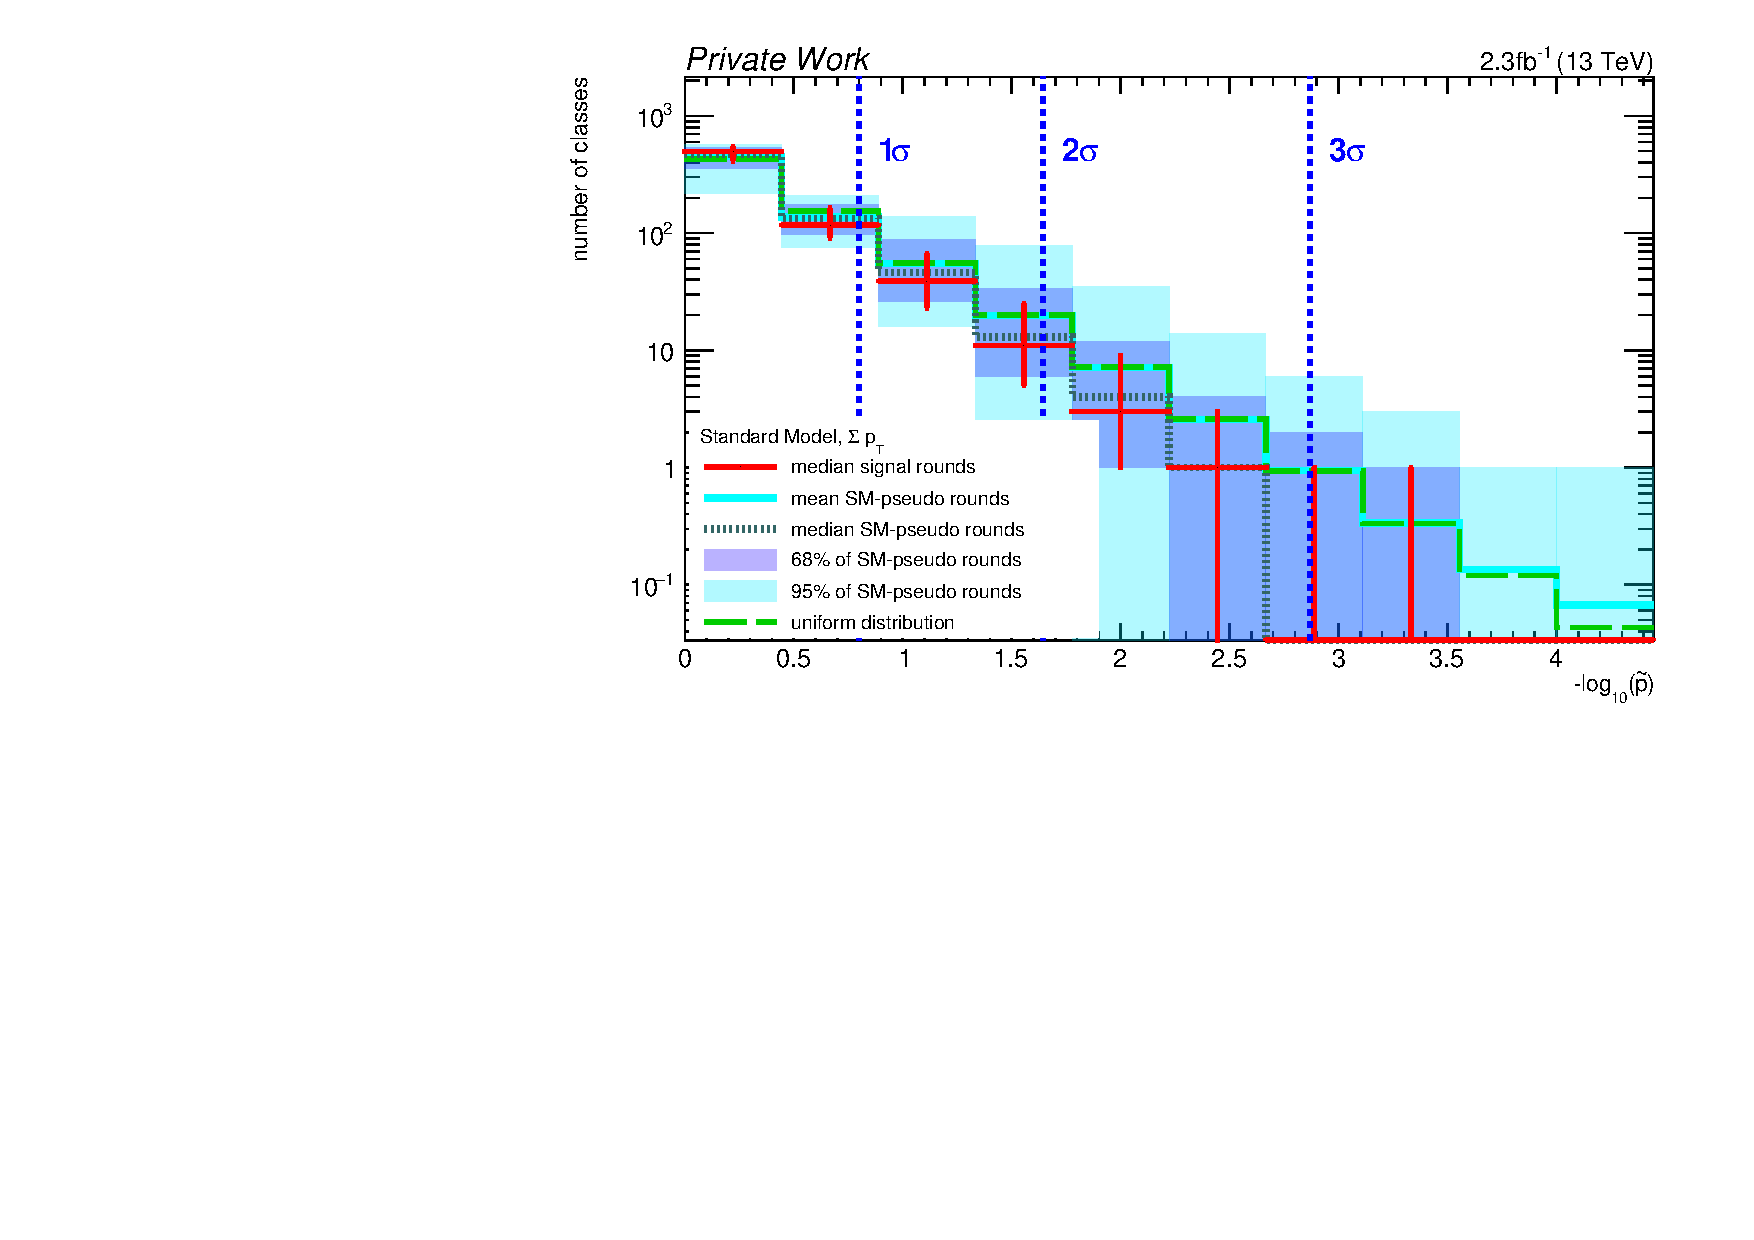
\includegraphics[width=\textwidth]{results/ptildeplots/signal,validation,bJets,SumPt/SM,bJets,SumPt/exclusive/pdf/p-tildeSumPt}
    \caption{Most significant classes for the \ac{QBH} model at $M = \SI{4000}{\GeV}$.}
\end{figure}
%
%
%\subsection{Black Holes}
%\subsubsection{Most Significant Classes}
%\begin{table}
%    \centering
%    \begin{longtable}{l S[table-figures-integer=1,table-figures-decimal=2,table-comparator=true,table-figures-exponent=1] S[table-figures-integer=1,table-figures-decimal=1,table-comparator=true,table-figures-exponent=0]}
\toprule
{Event Class} & {Median \ptilde} & {$Z$} \\
\midrule
\endhead
\num{1} \Pe + \num{1} \Pmu + \MET + X & 2.00e-04 & 3.5 \\
\num{1} \Pe + \num{1} \Pmu + X & 5.00e-04 & 3.3 \\
\num{1} \Pe + X & 1.82e-02 & 2.1 \\
\num{1} \Pe + \num{1} \Pmu + \num{1} jet + \MET + X & 4.39e-02 & 1.7 \\
\num{1} \Pe + \num{1} \Pmu + \num{1} jet + X & 1.47e-01 & 1.1 \\
\num{1} \Pe + \MET + X & 1.50e-01 & 1.0 \\
\num{1} \Pe + \num{1} \Pmu + \num{2} jets + \MET + X & 3.48e-01 & 0.4 \\
\num{1} \Pe + \num{1} \Pphoton + X & 3.74e-01 & 0.3 \\
\num{2} \Pe + \num{1} \Pmu + \num{1} \Pphoton + \MET + X & 3.74e-01 & 0.3 \\
\num{1} \Pe + \num{1} \Pphoton + \num{3} jets + \MET + \num{2} b-jets + X & 3.93e-01 & 0.3 \\
\bottomrule
\end{longtable}
%    \caption{Most significant classes for the \ac{QBH} model at $M = \SI{4000}{\GeV}$.}
%\end{table}
%
%\subsubsection{Distribution of \ptilde Values}
%\subsubsection{\phat Results}
%
%\subsection{Seesaw}
%
%\subsection{\PWprime}
%

\begin{figure}
    \centering
    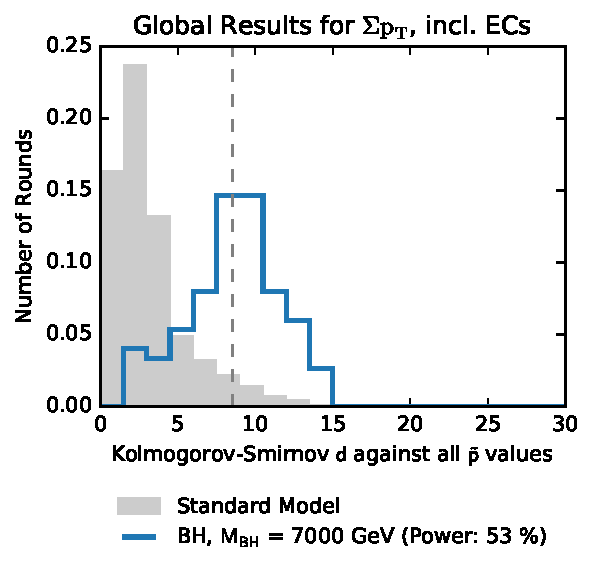
\includegraphics[width=0.5\textwidth]{results/phatplots/bJets/VALIDATION/exclusive/SumPt/KS_referenced_results}
    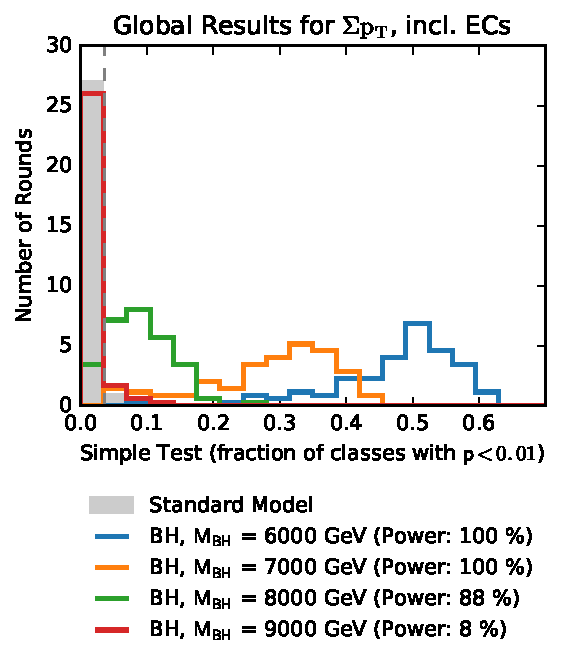
\includegraphics[width=0.5\textwidth]{results/phatplots/bJets/VALIDATION/exclusive/SumPt/Simple_results}
    \caption{\phat results for the validation. As expected, the test power of the null-hypothesis is about \SI{5}{\percent} and no significant deviation from the solid curve can be found.}
\end{figure}

\subsubsection{Differences between Luminosity of \SI{2.3}{\per\femto\barn} and \SI{35.9}{\per\femto\barn}}

\section{Discussion}


Concerning the choice of test statistic for \phat: It all cases, it seems that the simple test, which only counts very significant classes, outperforms more sophisticated test statistics which also perform a comparison in the bulk of the distribution. One possible explanation could be that the analysis has previously been developed with sensitivity towards very significant classes rather than optimizing for the bulk of the \ptilde distribution.
Nevertheless, the test power towards the other test statistics should be considered during future design decisions of the analysis.

\subsection{Comparison to dedicated analyses}
\begin{table}
    \centering
    \begin{tabular}{r r r r r r r}
        \toprule
        & \phantom{ab} & \multicolumn{2}{c}{$\mathcal{L} \approx \SI{2.3}{\per\femto\barn}$} & \phantom{ab} & \multicolumn{2}{c}{$\mathcal{L} \approx \SI{35.9}{\per\femto\barn}$} \\
        \cmidrule{3-4} \cmidrule{6-7}
        Model && \ac{CMS} Limit & \ac{MUSiC} && \ac{CMS} Limit & \ac{MUSiC} \\
        \midrule
        %RPV-SUSY $\lambda = 0.01$& \SI{1}{\TeV}\cite{CMS:CMS-PAS-EXO-16-001} & \SI{1.9}{\TeV}\tablefootnote{not public} & 0 \\
        QBH $n=4$ && \SI{4.2}{\TeV}\cite{CMS:CMS-PAS-EXO-16-001} & 0 && \SI{5.4}{\TeV}\tablefootnote{not public} & 0 \\
        Black Hole && \SI{8.6}{\TeV}\cite{CMS:CMS-PAS-EXO-15-007} & 0 && - & 0 \\
        Seesaw && \SI{440}{\GeV}\cite{CMS:CMS-PAS-EXO-16-002} & 0 && \SI{790}{\GeV}\cite{CMS:CMS-PAS-EXO-17-006} & 0 \\
        $\PWprime \to \Pqt \Pqb$ && \SI{2.4}{\TeV}\cite{CMSCollaboration:SearchesWbosons} & 0 && \SI{3.4}{\TeV}\cite{CMS:CMS-PAS-B2G-17-010} & 0 \\
        \bottomrule
    \end{tabular}
    \caption{Comparison of our discovery thresholds to comparable dedicated analyses published by the \ac{CMS} collaboration. Our values are the highest mass points at which \ac{MUSiC} is sensitive to the given model (according to the definition of \fref{sec:results}). Missing values indicate that the corresponding analysis on this model/luminosity combination has not been conducted.}
\end{table}

\subsection{General Validity for New Physics}

can the sensitivity be transferred towards unknown new physics?
pitfalls?